\documentclass[main.tex]{subfiles}

\begin{document}

\section*{Results}

The introduction of DRT across 60 scenarios consistently reduced aggregate daily congestion compared to the baseline scenario, where additional travel time incurred from delays constitutes the majority of total travel time. This aligns with findings by \cite{schluter2021impact}, who demonstrated significant reductions in congestion on rural-urban corridors through DRT implementations. Figure \ref{fig:x_6} illustrates the impact of DRT introduction on car use (measured by total cars on the road) and total congestion. The extent of reduction varied with DRT configuration, with scenarios featuring larger fleets and lower pricing achieving the greatest reductions, up to 28.2\,\% citywide. In the median scenario, congestion decreased by 12.7\,\%, while the least effective scenarios (e.g., smallest fleet sizes at highest prices) still yielded a modest 2.5\,\% reduction. This variability underscores that fleet size and pricing are critical levers for optimizing congestion relief potential of DRT, a point echoed by \cite{engelhardt2019quantifying} in their study on fleet optimization for shared mobility. Notably, even in less effective configurations, DRT contributed to decongestion, highlighting its robustness as a mitigation strategy. Scenarios with higher costs showed minimal shifts from car use, resulting in smaller congestion reductions, indicating that DRT's effectiveness hinges on its ability to compete with private cars on cost. Moreover, it is notable that the relative decrease in congestion often exceeds the reduction in the total number of cars on the street. This suggests that DRT not only reduces the number of vehicles but also enhances traffic flow efficiency. By optimizing routes, reducing stop-and-go traffic patterns, and potentially increasing vehicle occupancy through shared rides, DRT provides greater relief for remaining car users and improves overall traffic dynamics, a phenomenon also observed by \cite{maciejewski2016congestion} in their simulations of autonomous taxi fleets.

\begin{figure}[H]
\centering
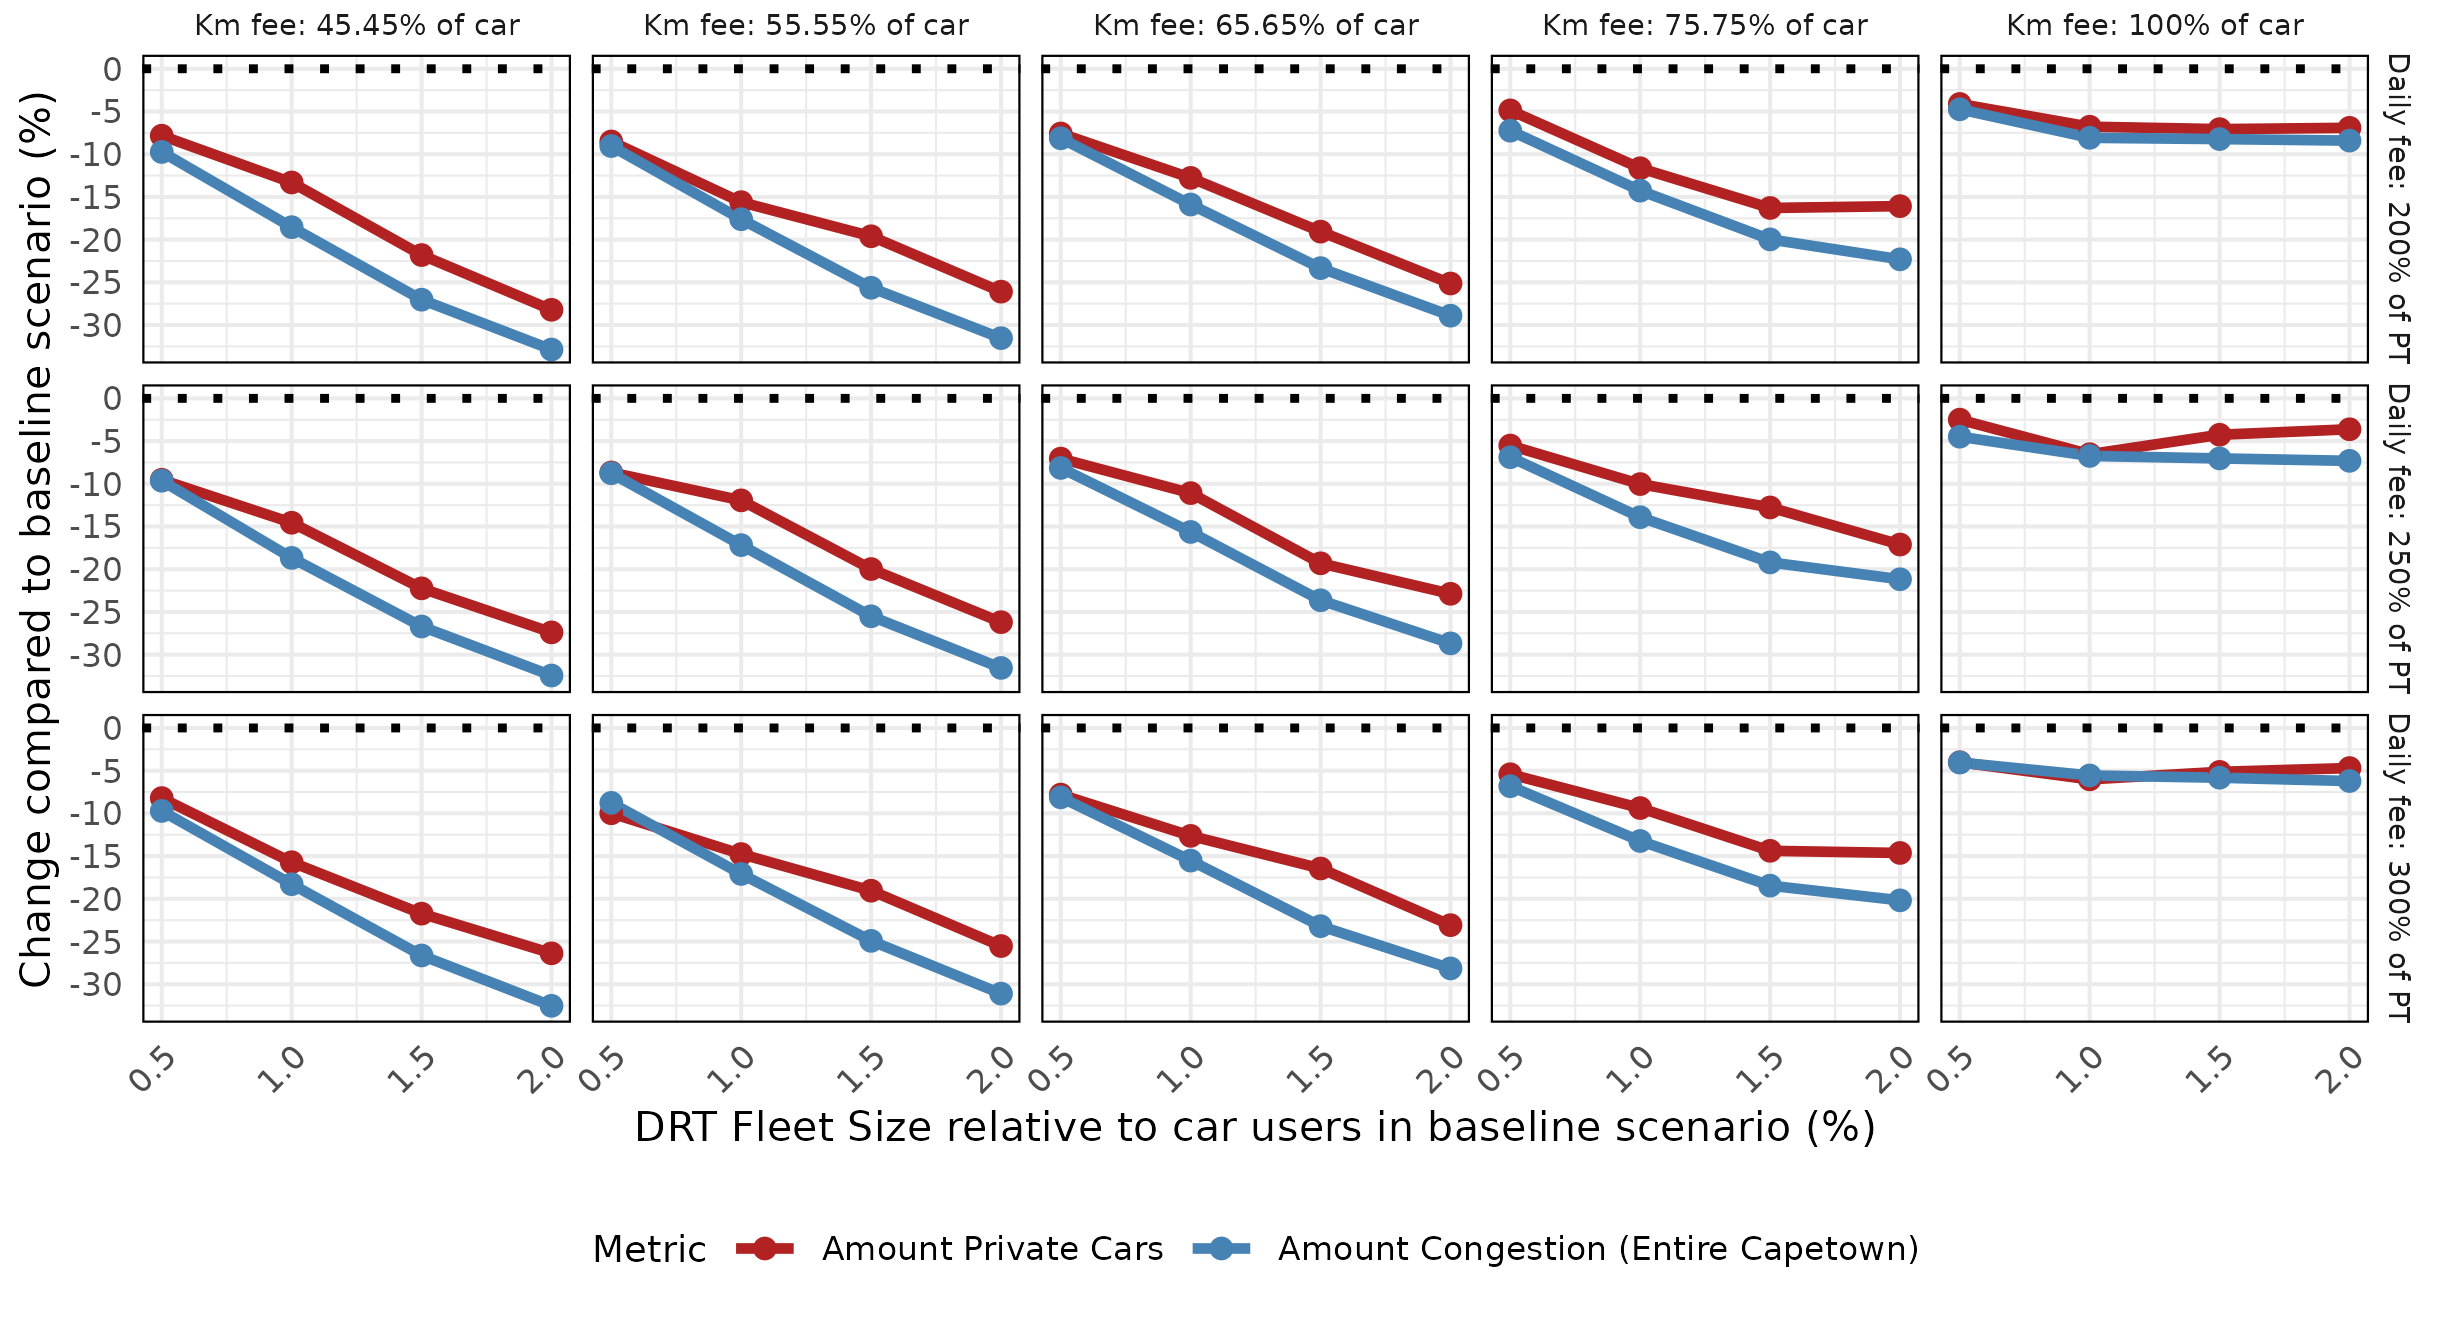
\includegraphics[width=0.9\textwidth]{images/drt_scenarios_grid_congestion_car_change_edit.png}
\captionsetup{width=.9\textwidth}
\caption{DRT introduction: Impact on car use and congestion}
\label{fig:x_6}
\end{figure}

Figure \ref{fig:x_10} shows the composition of change in congestion in different geographical areas in Cape Town. The buffer area, which likely serves as a transition zone between the DRT service area and outer regions, experiences the largest reduction, with congestion levels decreasing up to about 50\,\% in the most beneficial scenarios. This pronounced effect may be due to DRT alleviating traffic bottlenecks at the periphery of the service area, where vehicles often converge or disperse. In contrast, within the service area, congestion increases in the most expensive DRT scenarios, possibly because high prices deter adoption, leading to underutilization of DRT and a reliance on less efficient modes. However, this local increase is offset by reductions in other areas, resulting in overall congestion relief. Congestion reduction outside the service area is the smallest, though still positive, indicating that the impact of DRT extends beyond its immediate operational zone, likely through reduced through-traffic or altered travel patterns.

\begin{figure}[H]
\centering
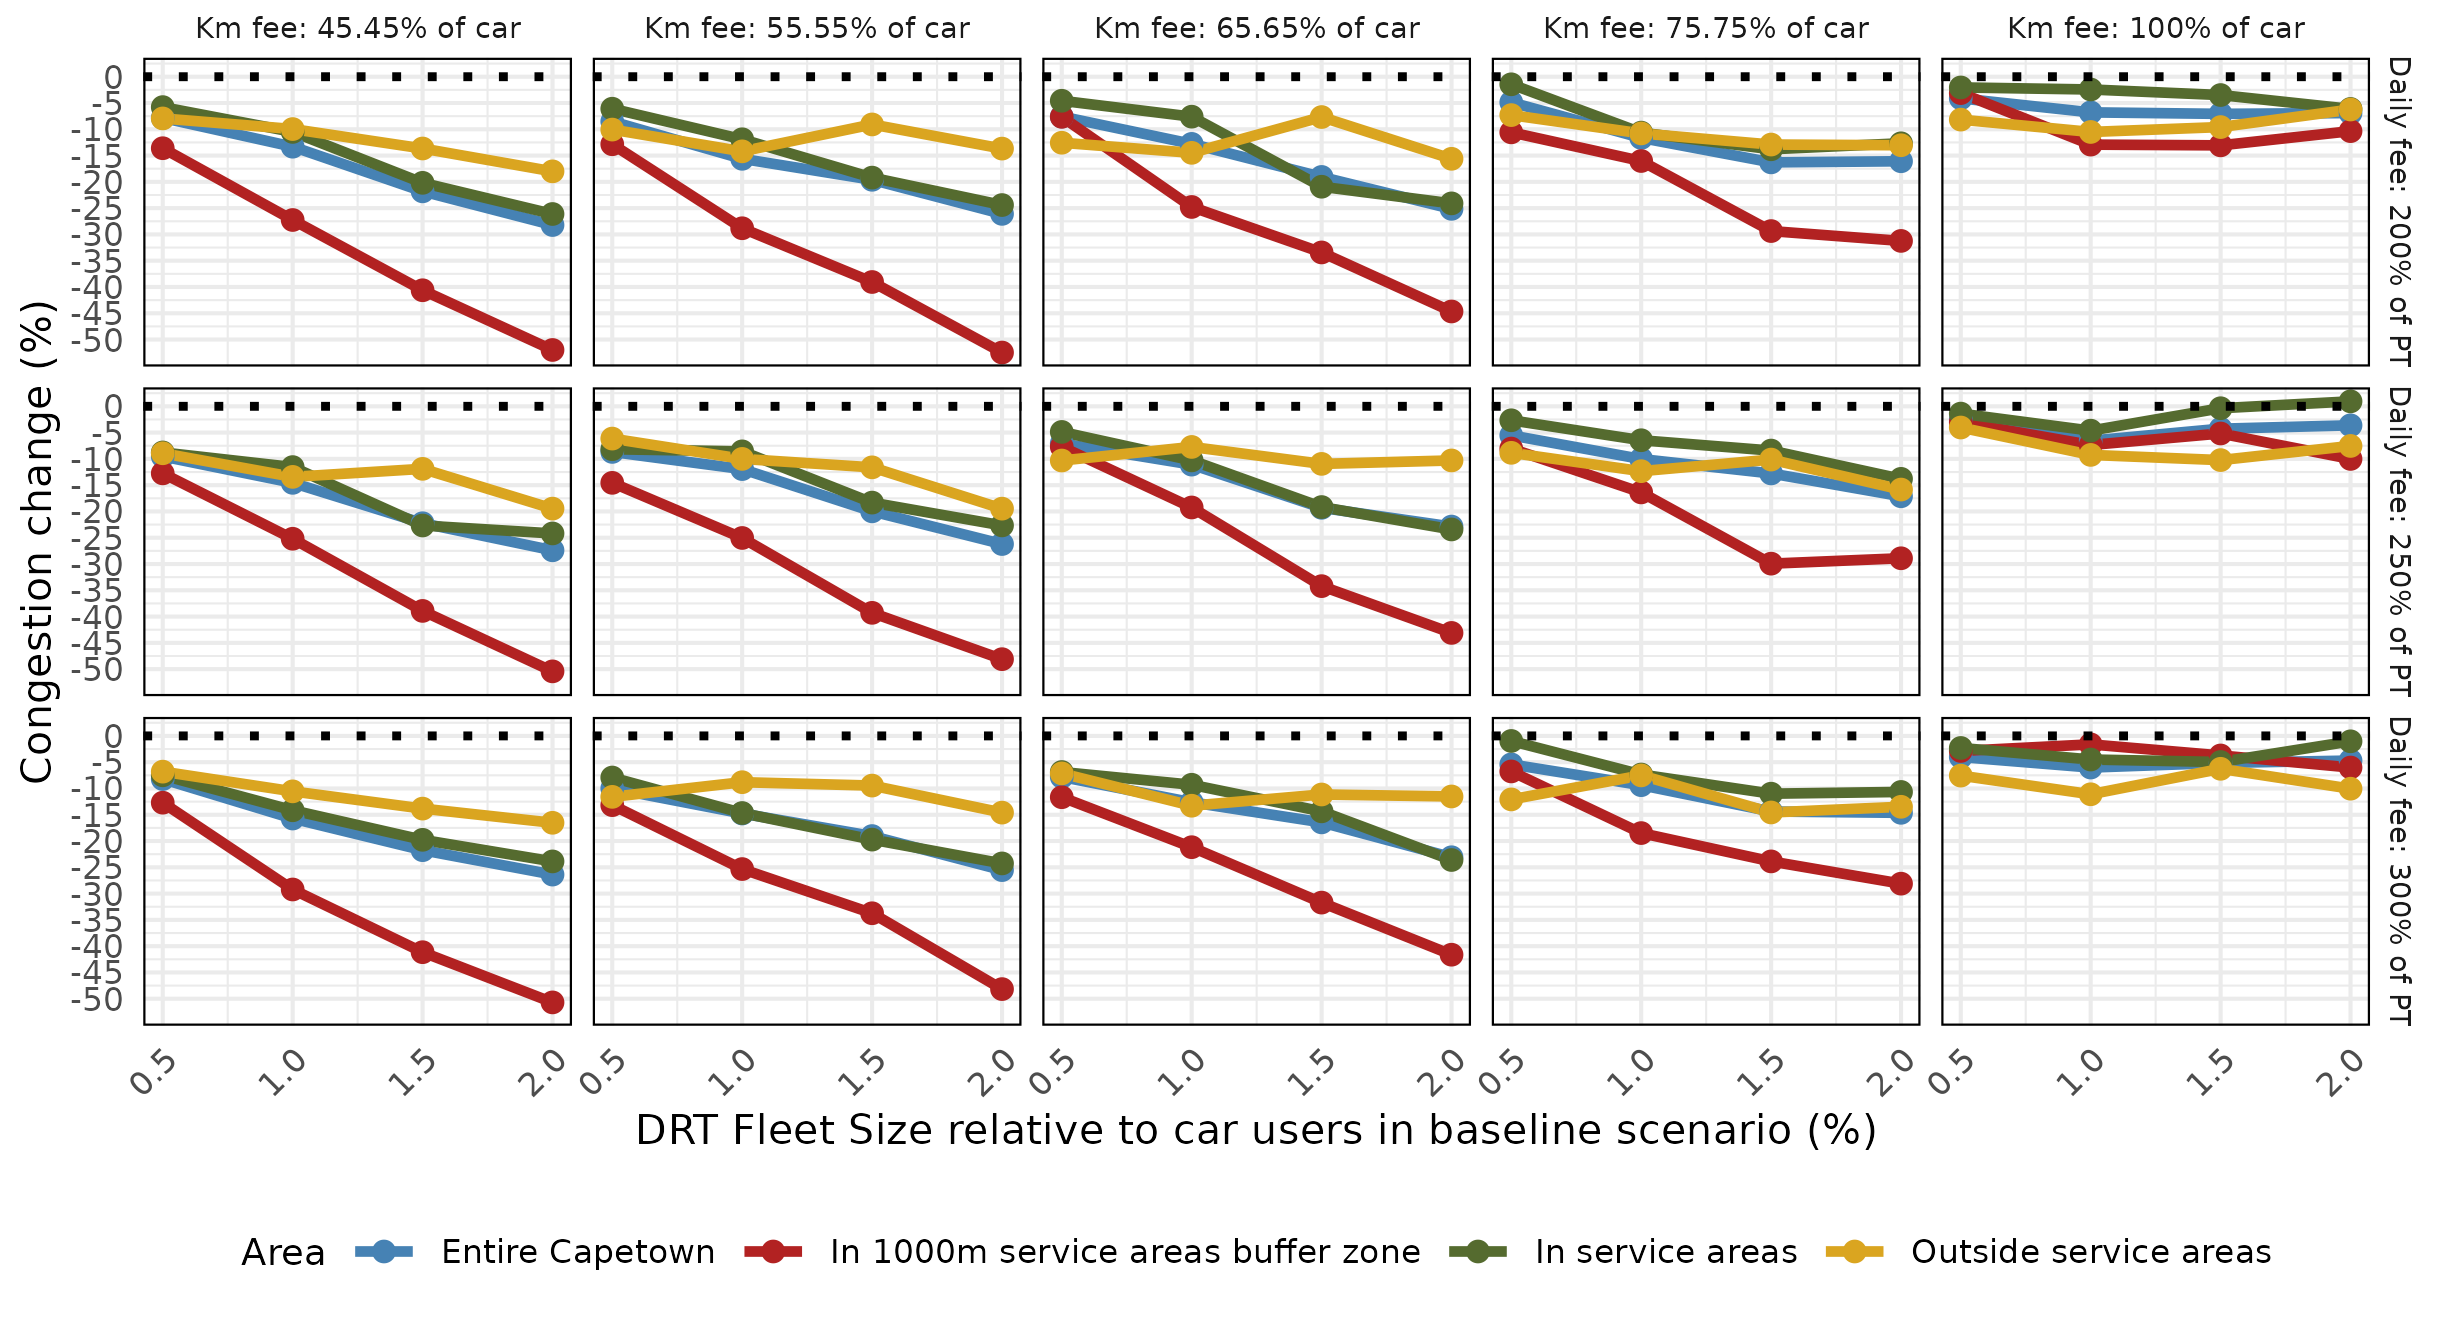
\includegraphics[width=.9\textwidth]{images/grid_congestion_different_areas_edit.png}
\captionsetup{width=.9\textwidth}
\caption{DRT introduction: Impact on congestion in different areas}
\label{fig:x_10}
\end{figure}

The introduction of DRT also altered the distribution of traveled kilometers across modes. In the baseline scenario, cars accounted for the majority of traveled kilometers (roughly 44\,\%). Figure \ref{fig:x_8} reveals that the introduction of DRT increases public transport mileage in all scenarios, possibly because DRT enables more flexible multi-modal trips. Previously, car users might have been constrained to use their cars for entire round-trip journeys to avoid leaving their vehicles at intermediate destinations; with DRT, they can switch modes more easily, potentially using public transport for parts of their trip. This observation is consistent with \cite{Kaddoura.2020b}, who found that DRT can act as a feeder service, enhancing public transport ridership. Additionally, car mileage decreases in all scenarios, with reductions of up to approximately 35\,\% in the most favorable configurations. However, the introduction of DRT also contributes to private motorized mileage through the operation of DRT vehicles themselves. In some scenarios, this addition may offset the reduction in car mileage, leading to a net increase in total private motorized mileage. Nevertheless, as observed in Figure \ref{fig:x_6}, congestion still decreases, suggesting that DRT vehicles are utilized more efficiently than private cars, potentially due to higher occupancy or improved routing.

\begin{figure}[H]
\centering
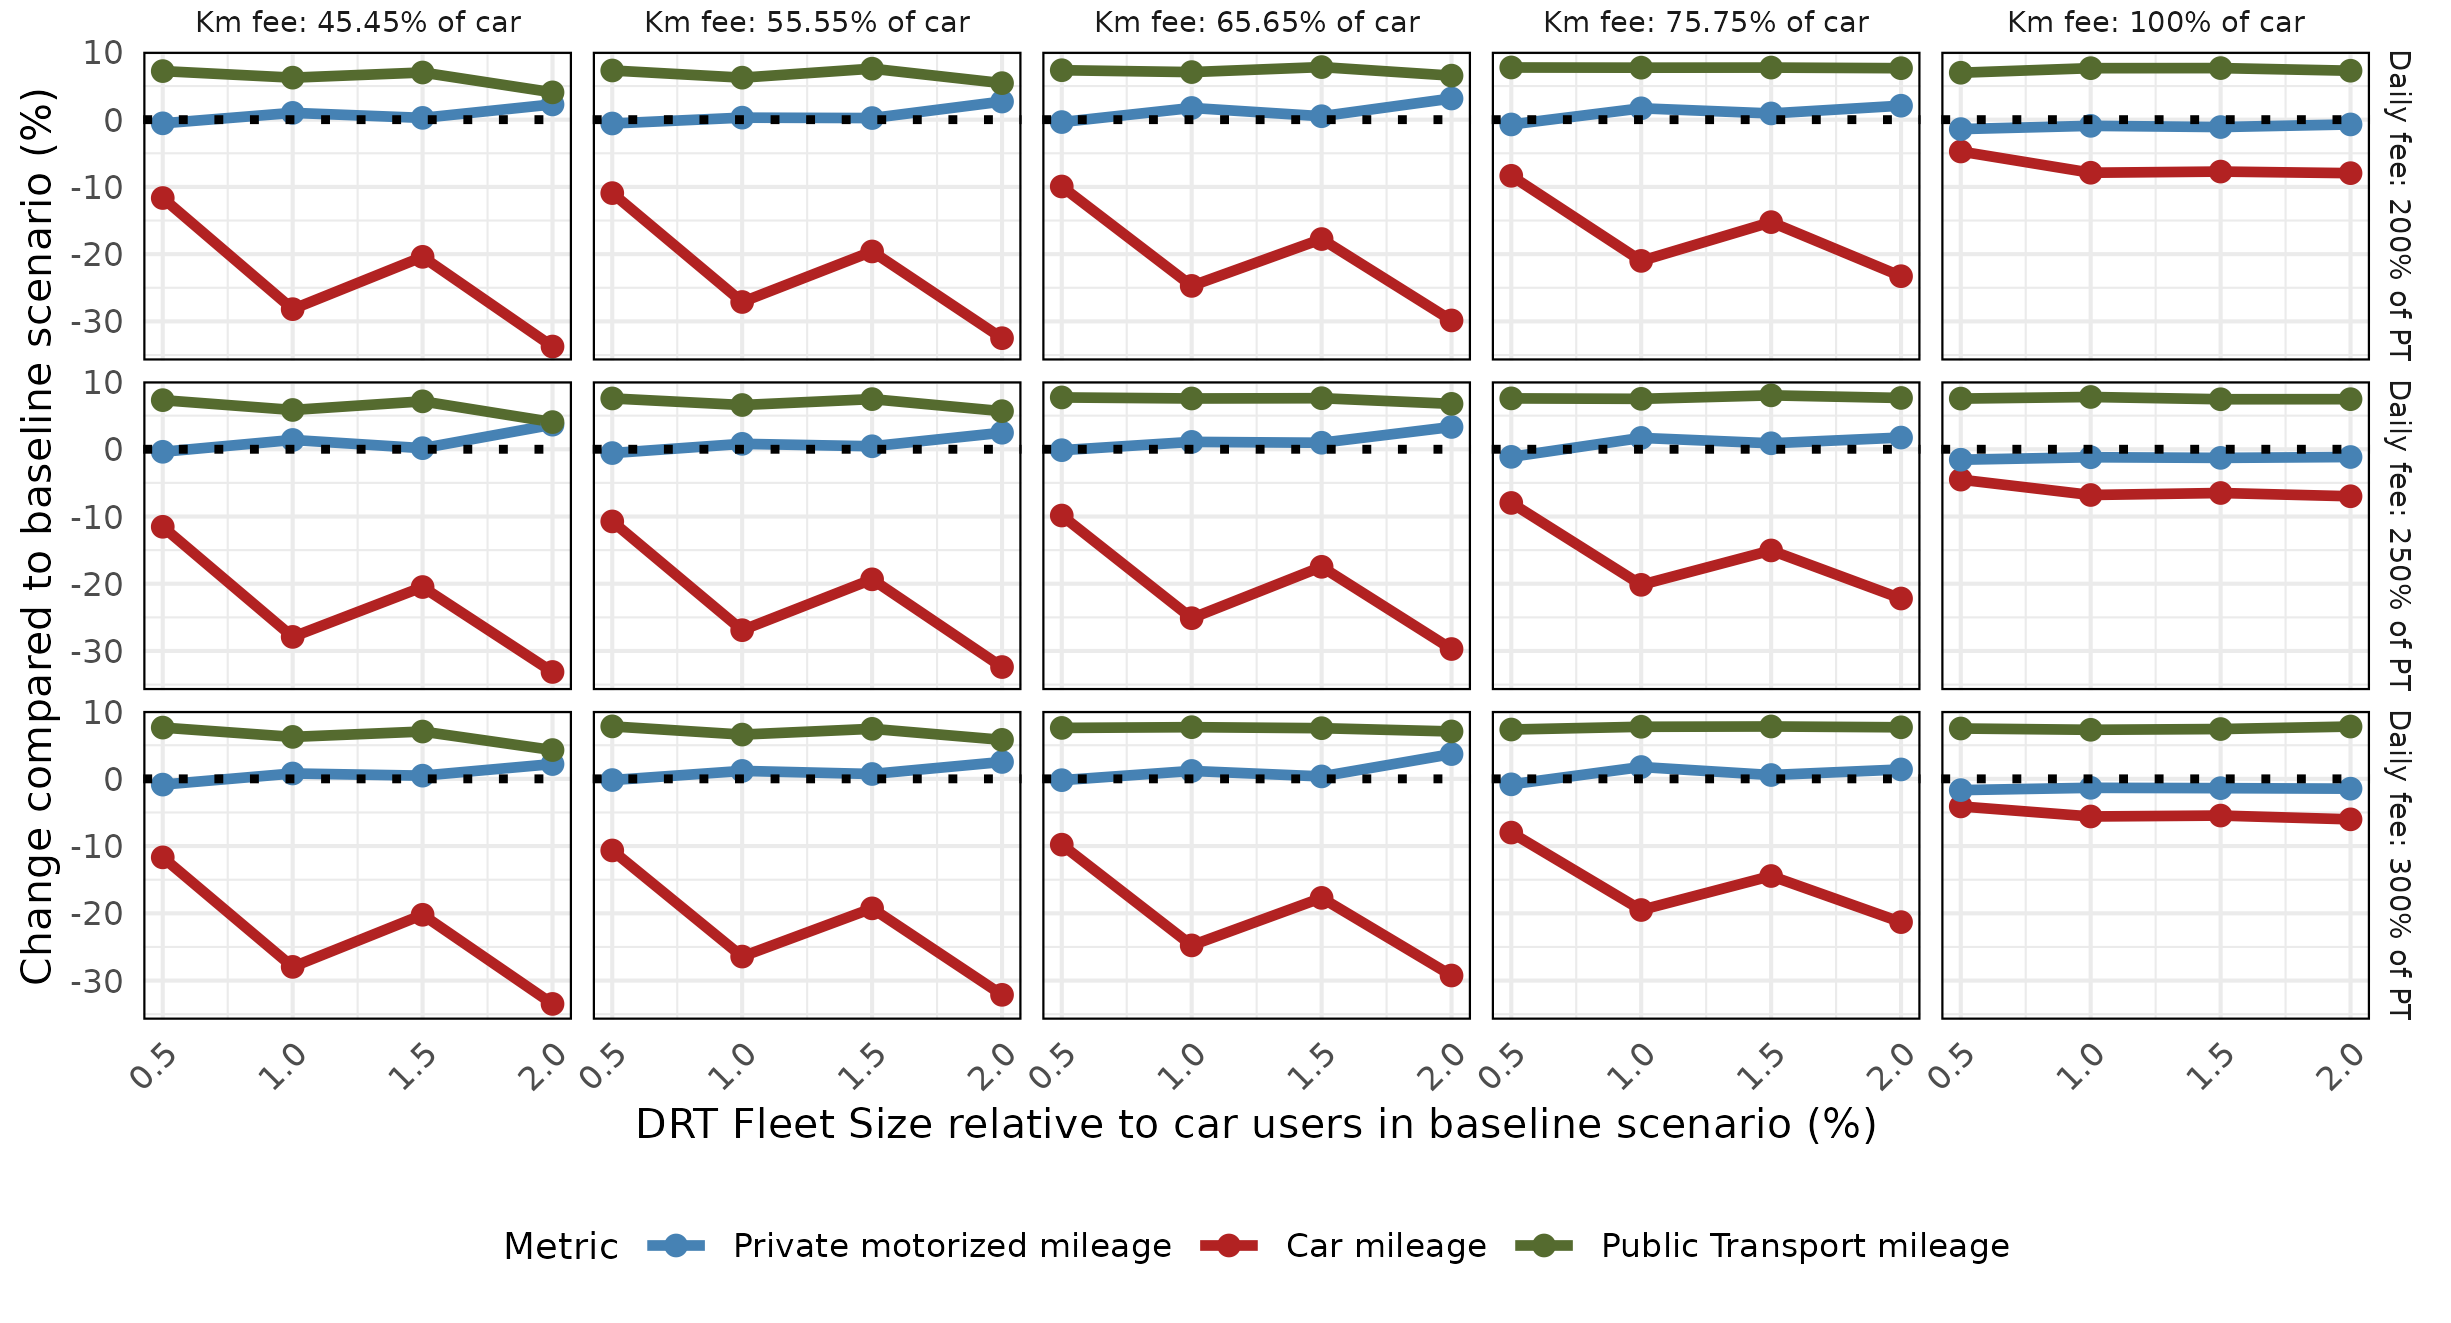
\includegraphics[width=.9\textwidth]{images/drt_mileage_edit.png}
\captionsetup{width=.9\textwidth}
\caption{DRT introduction: Impact on private motorized and public transport mileage}
\label{fig:x_8}
\end{figure}

The introduction of DRT also prompted notable shifts in mode choice. Figure \ref{fig:x_7} displays the relative occurrences of selected mode shifts across all mode changes in each scenario. There is no significant cannibalization of public transport by DRT. In most configurations, while larger DRT fleets attract some public transport users to switch to DRT, this is counterbalanced by a more substantial shift from car users to public transport, often resulting in a net increase in public transport usage. This finding aligns with \cite{miskolczi2021urban}, who noted enhanced connectivity in sustainable transport networks through DRT. At a fixed pricing level, fleet size has a negligible impact on the attractiveness of DRT for public transport users, suggesting that pricing plays a more critical role in mode choice for this group. For car users, an increase in DRT fleet size leads to a higher proportion of switches from cars to DRT, although this effect diminishes in scenarios with higher DRT pricing. Interestingly, in scenarios with the most expensive distance fares for DRT, the predominant mode switch is from cars to public transport, a favorable outcome for reducing car dependency. This suggests that when DRT is priced competitively, it directly attracts car users, whereas higher prices may encourage a shift toward public transportation instead. \textcolor{green}{Accordingly, it can be concluded when DRT is priced competitively, it directly attracts car users, whereas higher prices may encourage a shift toward public transportation instead.

\begin{figure}[H]
\centering
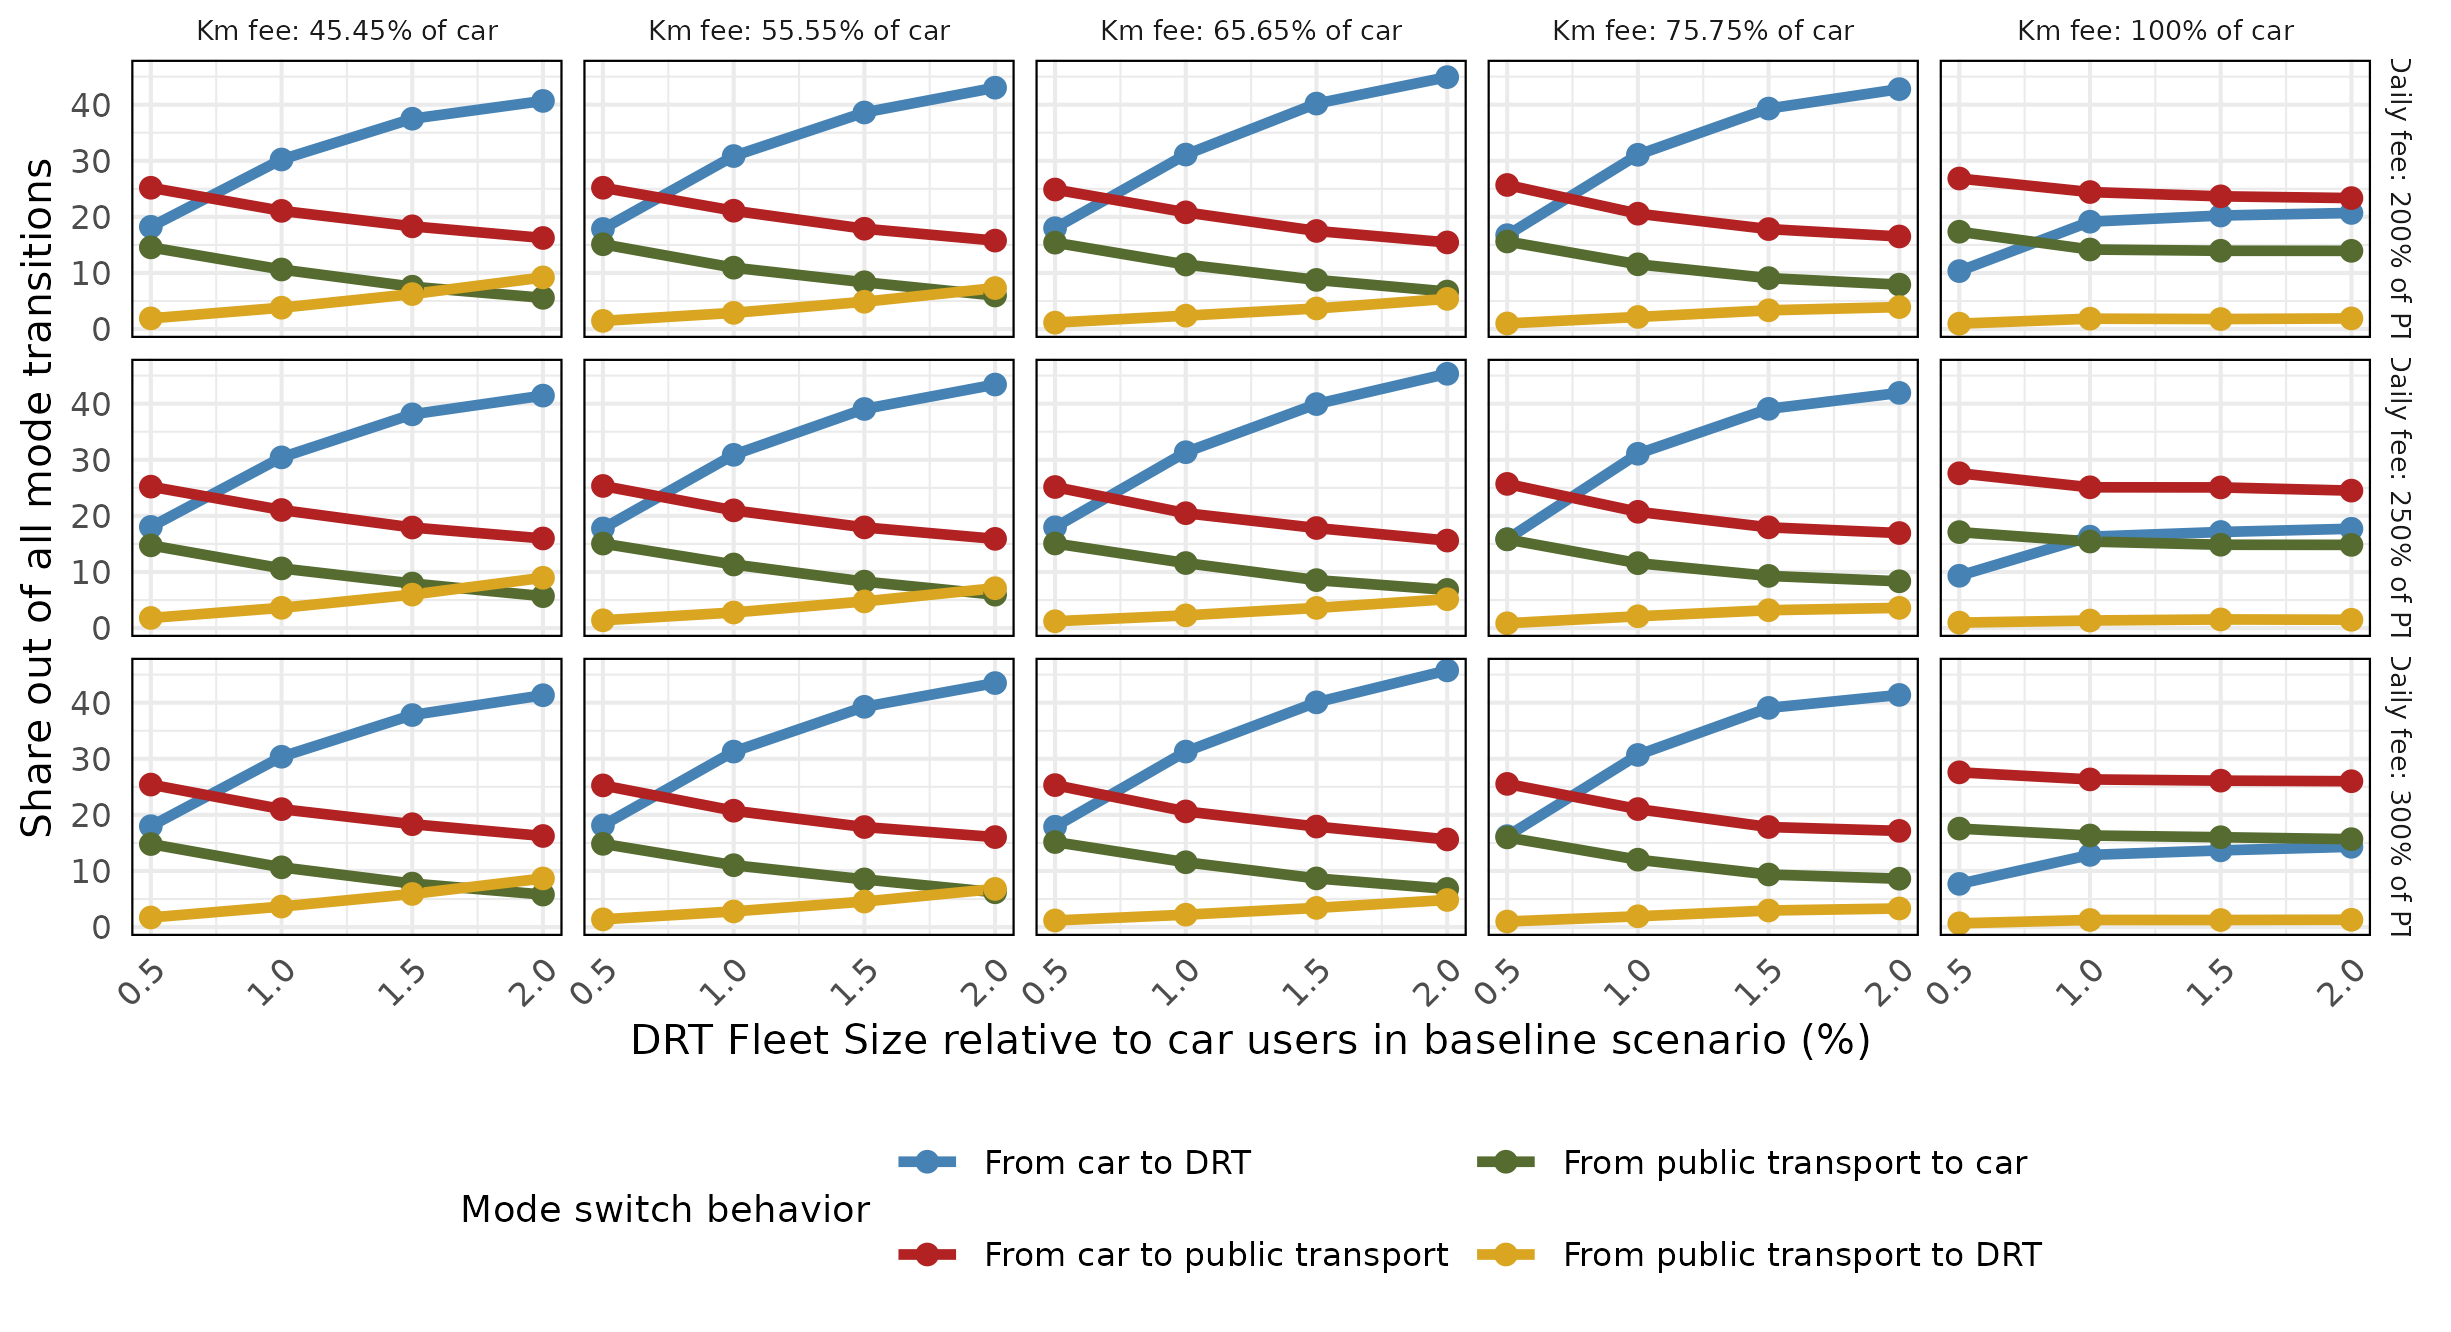
\includegraphics[width=0.9\textwidth]{images/drt_mode_switch_behavior_edit.png}
\captionsetup{width=.9\textwidth}
\caption{DRT introduction: Mode switch behavior}
\label{fig:x_7}
\end{figure}

Figure \ref{fig:x_9} presents the occupancy profiles of DRT vehicles, providing insight into their operational efficiency. The data indicate that additional mileage, or `dead mileage', accounts for roughly 10\,\% of DRT vehicle kilometers, representing the distance traveled without passengers during reallocation. However, shared rides, where multiple passengers are transported simultaneously, constitute between 25\,\% and 40\,\% of DRT trips, depending on the pricing level. This suggests that the inefficiency introduced by dead mileage is largely offset by the efficiency gains from ride-sharing. Furthermore, even rides with a single passenger may involve detours to pick up additional passengers, thereby reducing the overall dead mileage per trip. These findings highlight the importance of optimizing DRT operations to maximize shared rides and minimize empty vehicle travel, which is crucial for enhancing the system's efficiency and environmental benefits, as also emphasized by \cite{engelhardt2019quantifying}.

\begin{figure}[H]
\centering
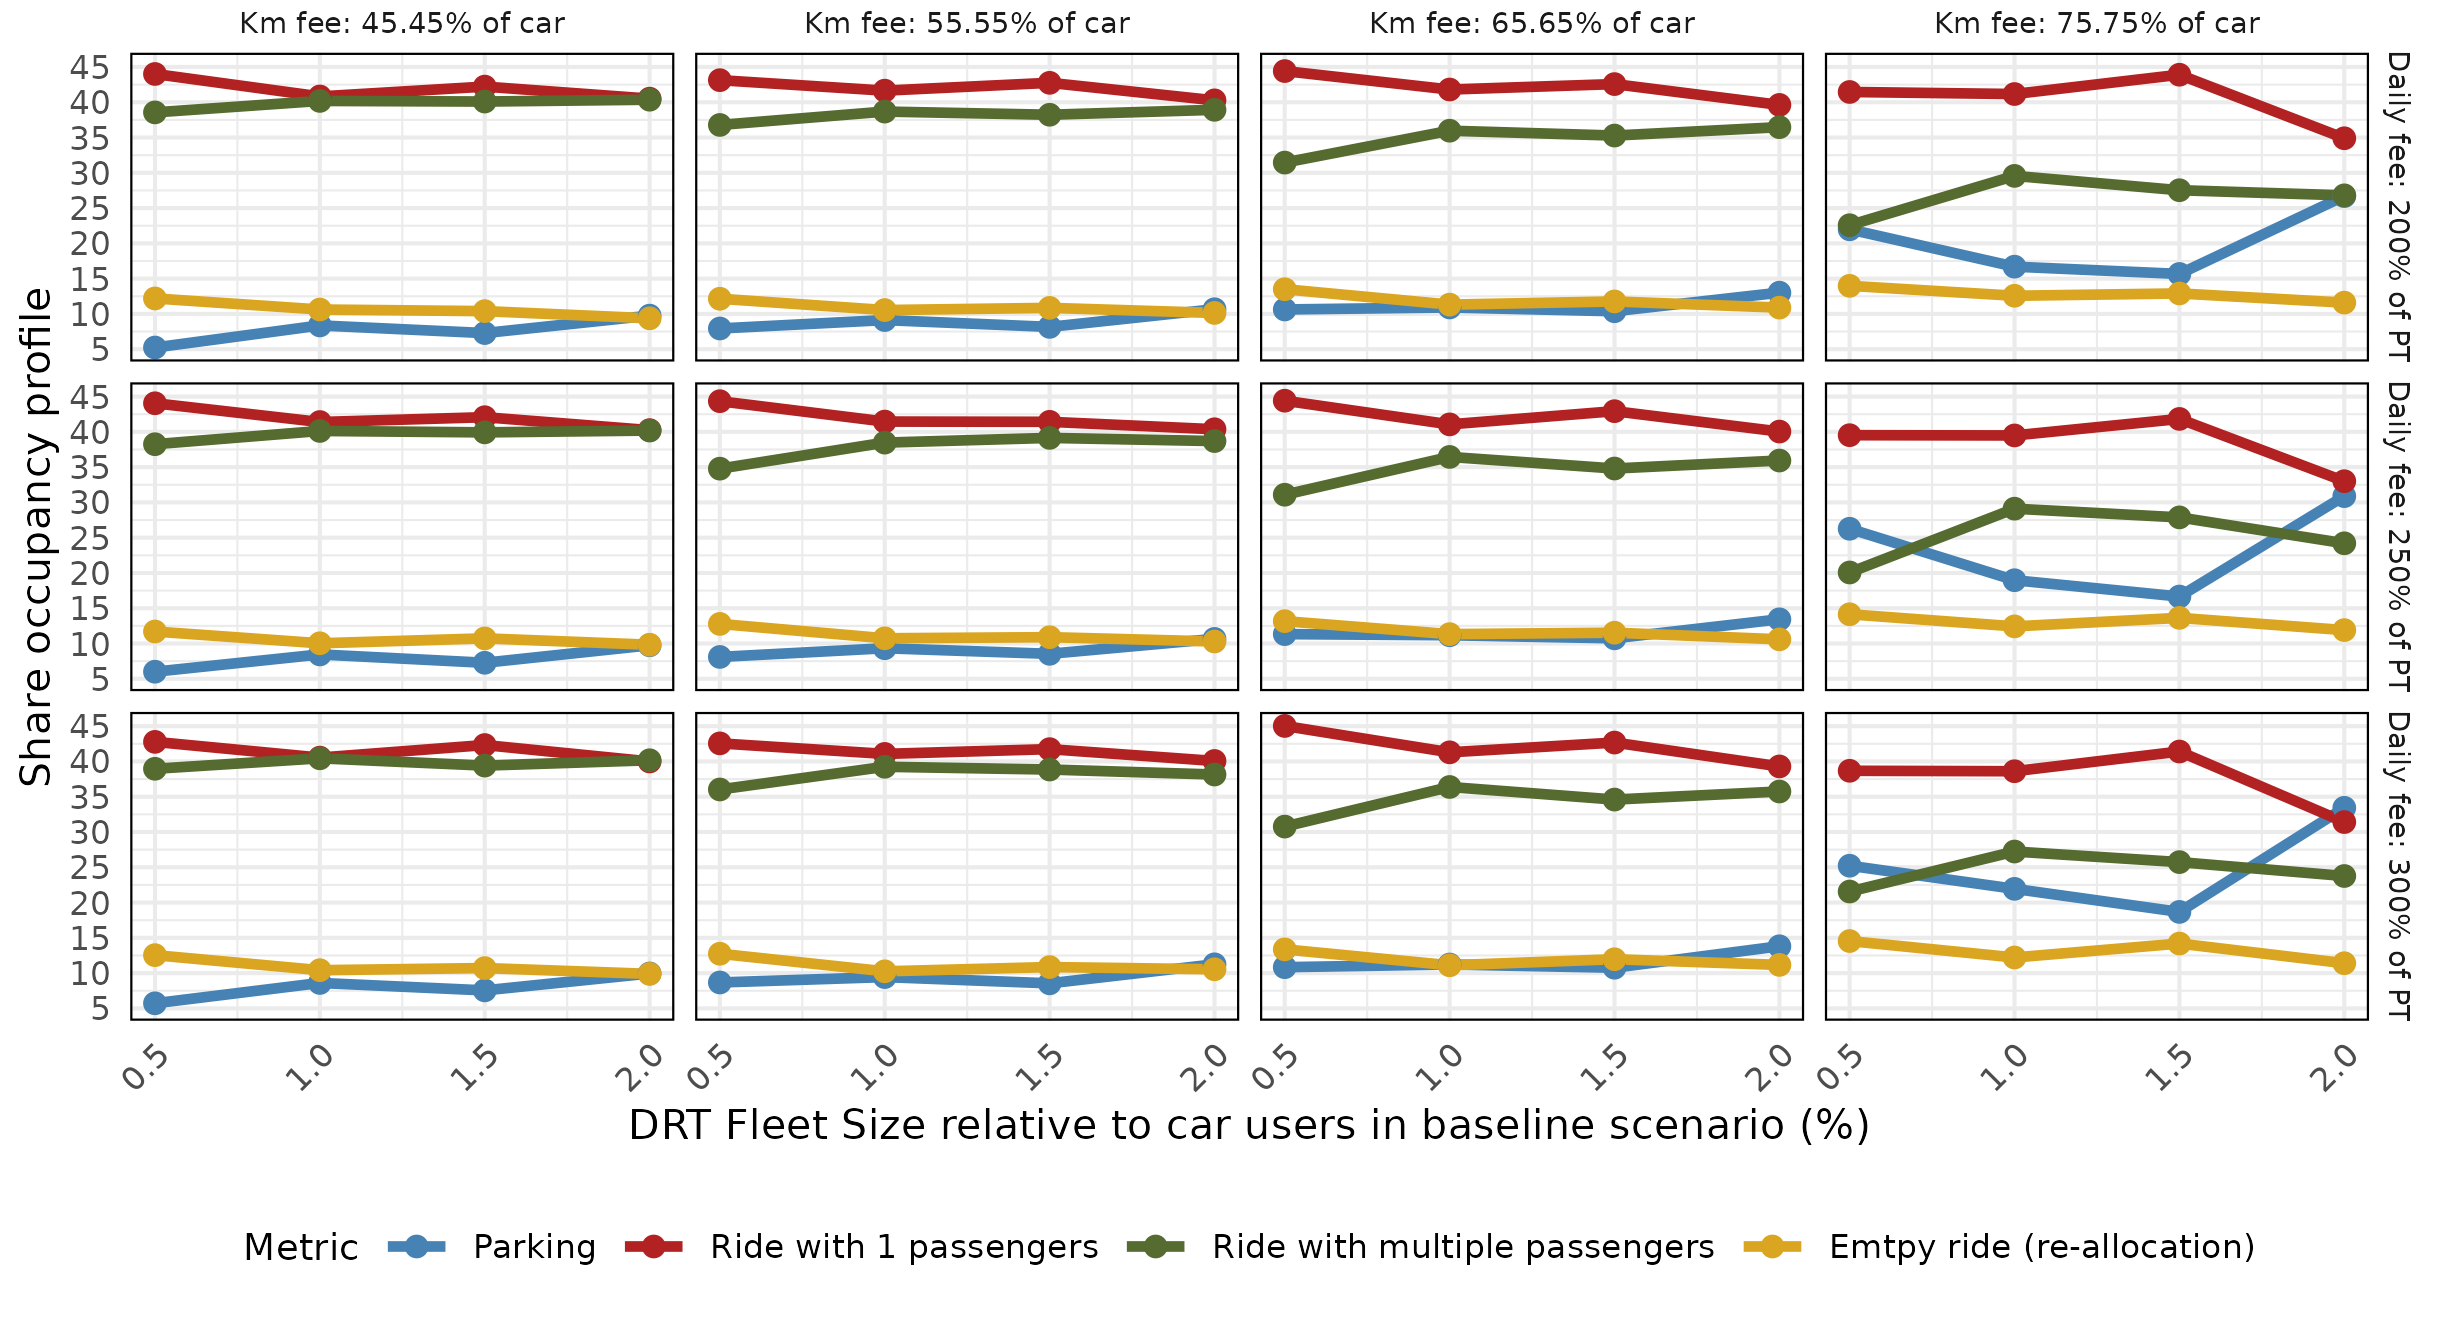
\includegraphics[width=0.9\textwidth]{images/drt_occupancy_grid_edit.png}
\captionsetup{width=.9\textwidth}
\caption{DRT introduction: Occupancy profiles of DRT vehicles}
\label{fig:x_9}
\end{figure}

To better analyze the effect of DRT on congestion and travel behavior in Cape Town, we focus on the scenario configuration with the overall congestion reduction closest to the median value. This scenario, which serves as a representative case, involves a DRT fleet size equal to 1\,\% of total car users (528 vehicles in our 10\,\% sample simulation), a distance kilometer fee equal to 59.1\,\% of the car equivalent, and a daily fee double that of public transport. Figure \ref{fig:x_11} shows the spatial distribution of congestion changes in this scenario, with the DRT service area overlayed. Notably, the Central Business District (CBD) exhibits a substantial reduction in absolute congestion, with a daily decrease of roughly 2000 hours, corresponding to a 41\,\% reduction compared to the baseline. This significant improvement in the CBD underscores the potential of DRT to alleviate congestion in high-traffic urban cores, where the concentration of trips and limited road capacity often lead to severe bottlenecks.

\begin{figure}[H]
\centering
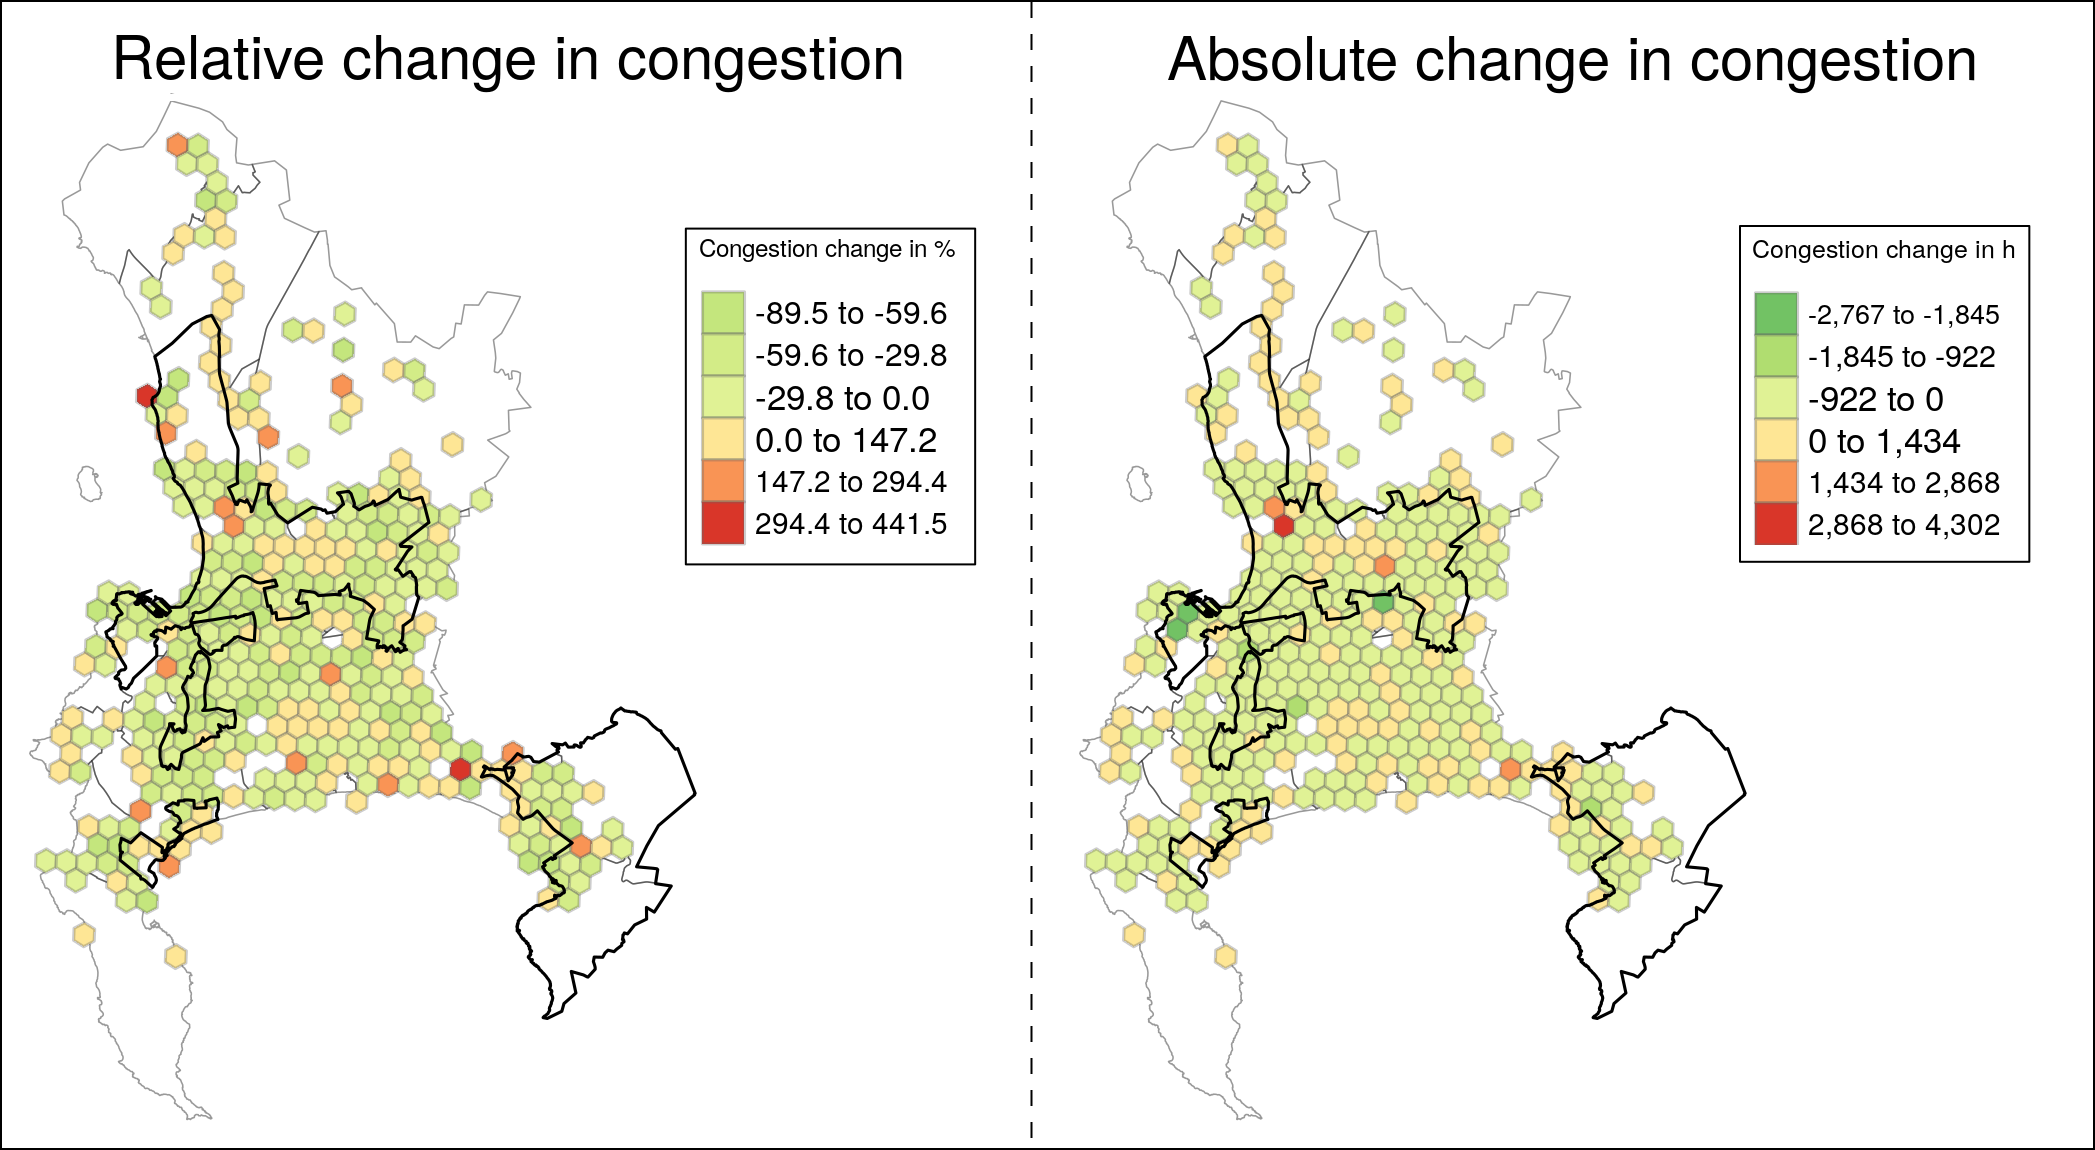
\includegraphics[width=0.9\textwidth]{images/median_scenario_congestion_map_edit_3.png}
\captionsetup{width=.9\textwidth}
\caption{Median DRT scenario: absolute and relative change in congestion. The bold areas mark the DRT service area constructed}
\label{fig:x_11}
\end{figure}

The introduction of DRT also impacted travel times across different modes and geographic areas, a key factor influencing user experience and mode choice. Figure \ref{fig:x_12} illustrates the median travel time changes for car and public transport trips in the median DRT scenario compared to the baseline. Across all geographic regions, median car travel times decreased significantly, with reductions ranging from 12 to 17 minutes. This aligns with the substantial congestion reductions observed in Figure \ref{fig:x_6} and Figure \ref{fig:x_10}, particularly in the buffer area (up to 50\,\% reduction), where alleviated bottlenecks likely contribute to faster car trips. For public transport, the effects are mixed. Trips with an origin or destination within the DRT service area saw median travel times reduced by nearly 15 minutes, possibly due to decreased road congestion benefiting bus and minibus operations, as seen in the CBD’s 41\,\% congestion reduction (Figure \ref{fig:x_11}). However, public transport trips in or between service areas experienced an increase in median travel time by approximately 15 minutes. This increase may stem from heightened demand for public transport, driven by mode shifts from cars (Figure \ref{fig:x_7}), which could overload routes or lead to longer waiting times. Additionally, in expensive DRT scenarios, increased congestion within service areas (Figure \ref{fig:x_10}) may delay public transport vehicles, further contributing to extended travel times. These findings suggest that while DRT enhances travel efficiency for cars and some public transport users, operational challenges in high-demand service areas require attention to maintain public transport reliability. Similar mixed results on travel times have been reported by \citep{reck2020shared}, who noted that public transport impacts vary depending on integration levels.

\begin{figure}[H]
\centering
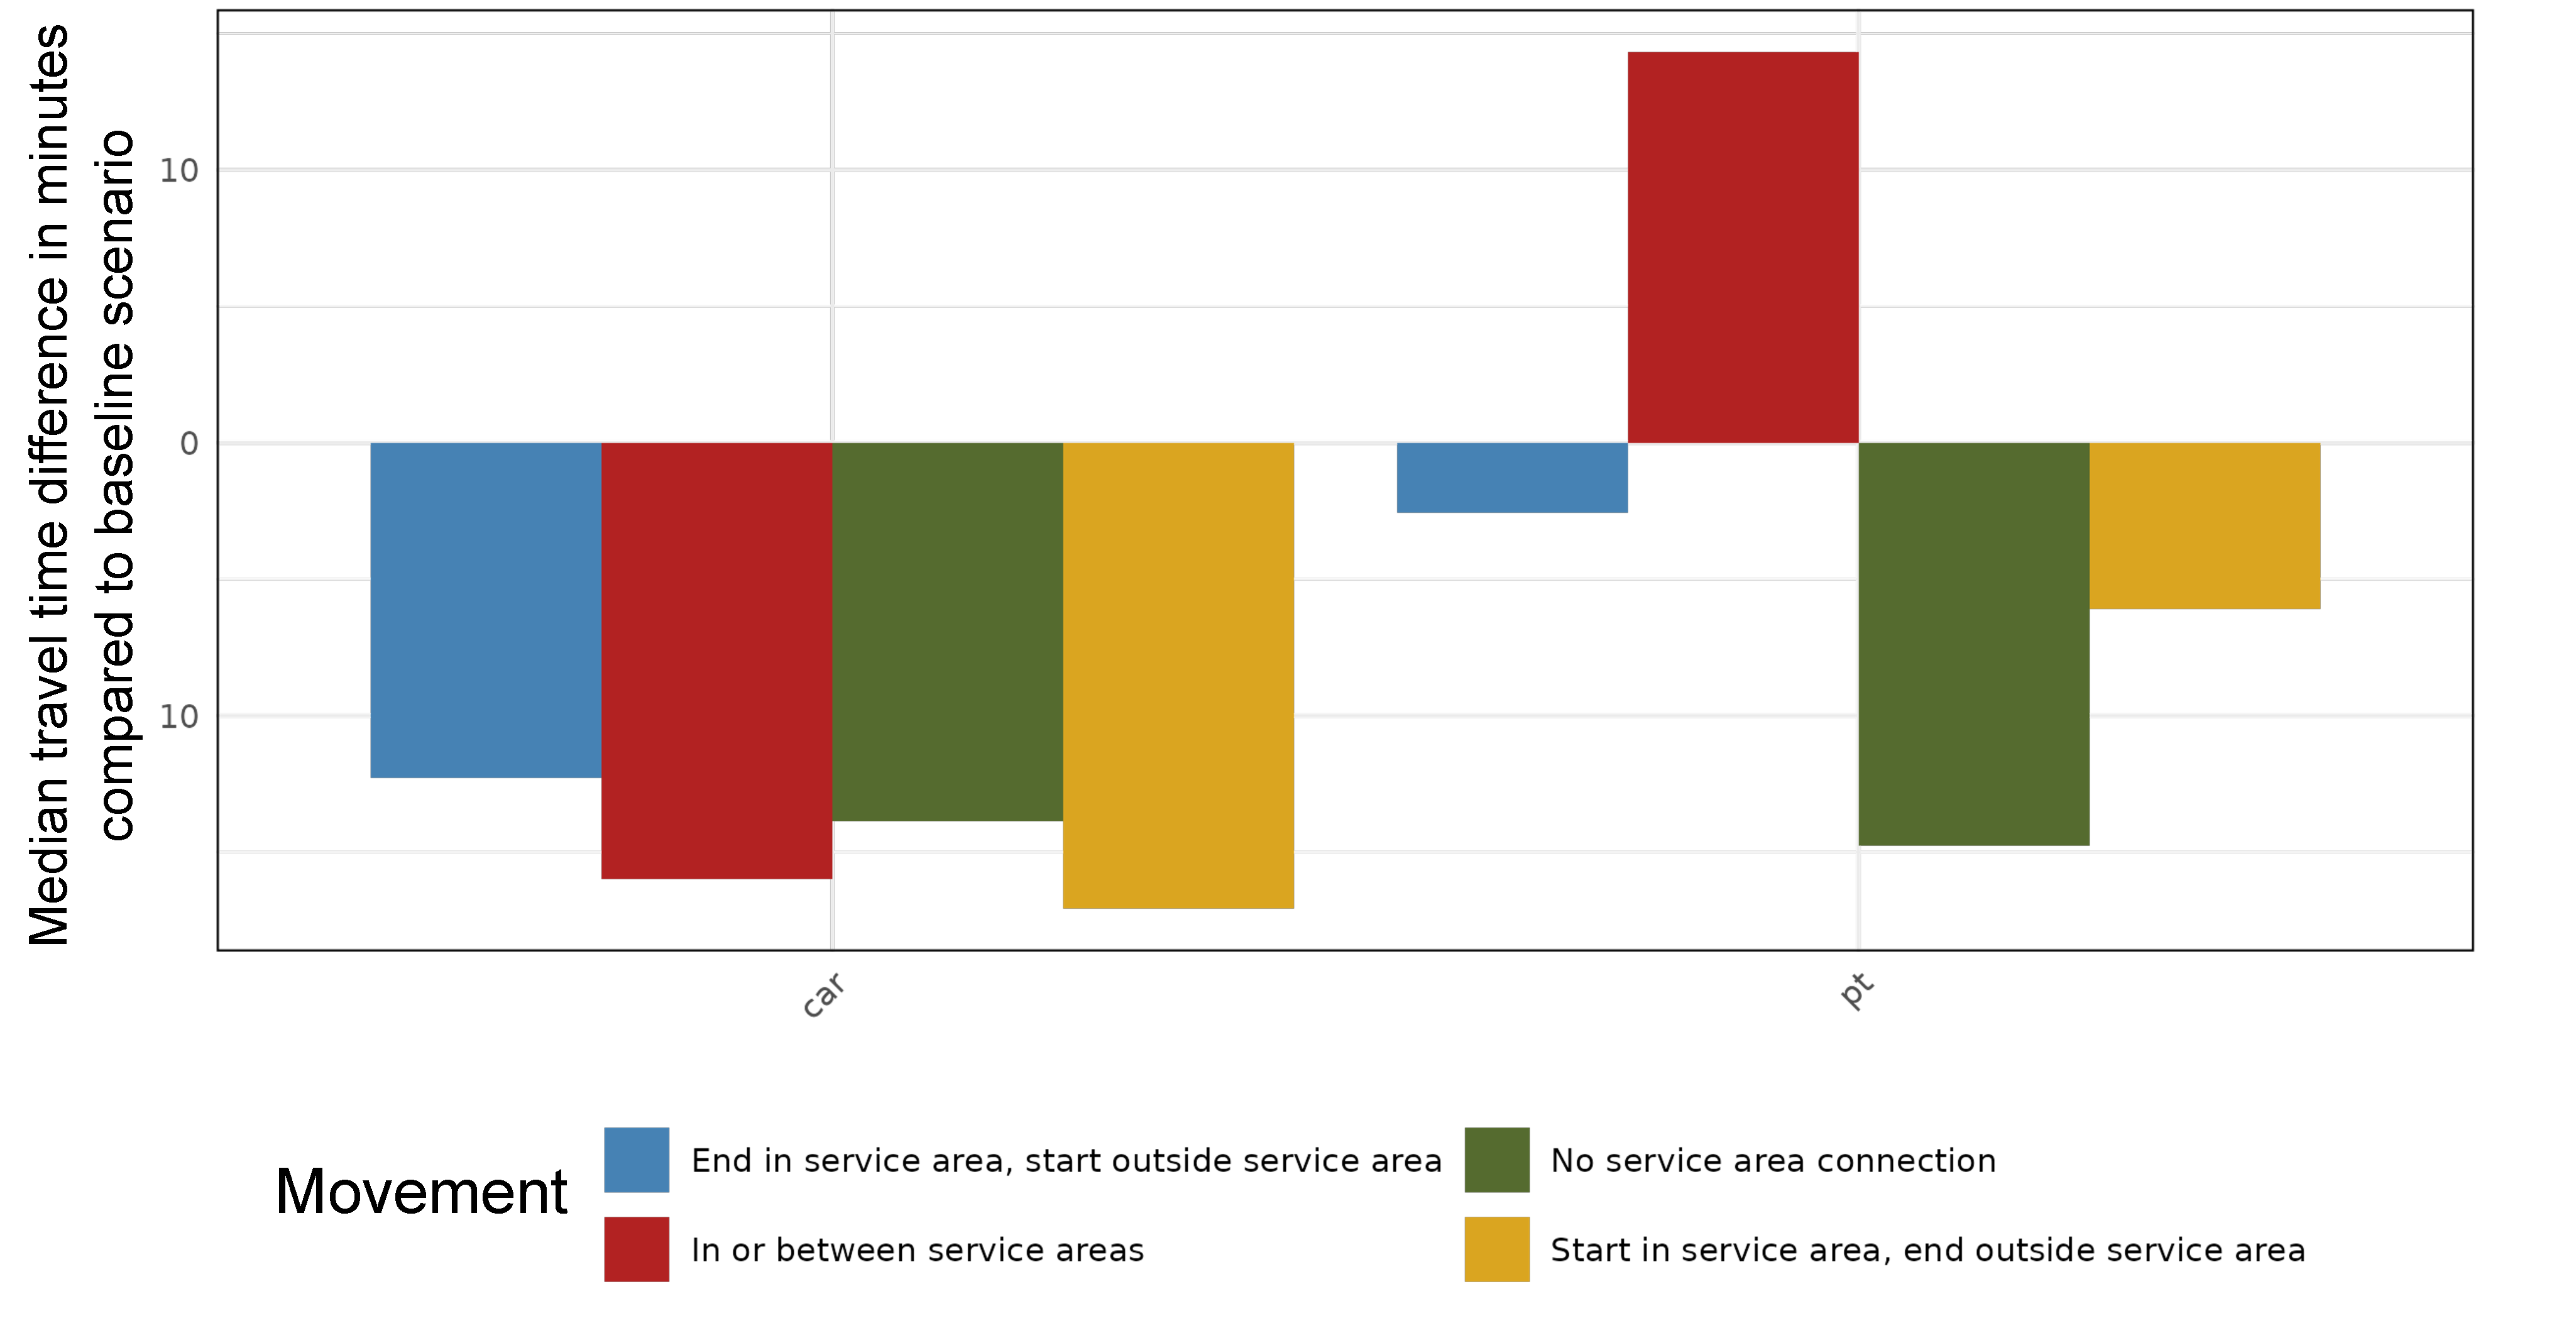
\includegraphics[width=0.9\textwidth]{images/median_scenario_pt_car_travel_time_change_edit.pdf}
\captionsetup{width=.9\textwidth}
\caption{Median DRT scenario: Median travel time for car and public transport before and after DRT introduction}
\label{fig:x_12}
\end{figure}

%\textcolor{red}{Is the effect of ride hailing considered in this model? this may likely impact the choice of simulated fleet sizes and prices.} \textcolor{}{see discussion/limitations.}

\end{document}